\documentclass[9pt,conference]{IEEEtran}
\usepackage[utf8]{inputenc}
\usepackage[T1]{fontenc}
\usepackage[stretch=10,shrink=20]{microtype}
\usepackage{graphicx}
\usepackage{booktabs}
\usepackage{amsmath,amssymb,amsfonts}
\usepackage{textcomp}
\usepackage{xcolor}
\usepackage{tikz}
\usepackage{pgfplots}
\pgfplotsset{compat=1.18}
\usetikzlibrary{shapes.geometric,arrows.meta,positioning,fit,backgrounds,shadows,
                decorations.pathreplacing,decorations.markings,calc,patterns,
                matrix,chains,scopes,shadings}

\usepackage{stfloats}
\usepackage[
    colorlinks=true,
    urlcolor=blue,
    linkcolor=blue,
    citecolor=blue,
    pdfborder={0 0 0}
]{hyperref}

\usepackage{geometry}
\geometry{
  letterpaper,
  top=0.30in, bottom=0.28in,
  left=0.38in, right=0.38in,
  columnsep=0.15in
}

\renewcommand{\baselinestretch}{0.91}

\setlength{\abovecaptionskip}{1pt}
\setlength{\belowcaptionskip}{-6pt}
\setlength{\textfloatsep}{0pt}
\setlength{\intextsep}{0pt}
\setlength{\dbltextfloatsep}{0pt}
\setlength{\parskip}{0pt}

% ---- colour palette ----
\definecolor{clBlue}{HTML}{1A3C5E}
\definecolor{clLightBlue}{HTML}{2E86C1}
\definecolor{clCyan}{HTML}{17A589}
\definecolor{clOrange}{HTML}{D35400}
\definecolor{clRed}{HTML}{C0392B}
\definecolor{clGreen}{HTML}{1E8449}
\definecolor{clPurple}{HTML}{6C3483}
\definecolor{clGold}{HTML}{B7950B}
\definecolor{clGray}{HTML}{5D6D7E}
\definecolor{clTeal}{HTML}{0E6655}

\begin{document}
\enlargethispage{3.2in}

\title{%
\textbf{Network Intrusion Detection System}\\
\large\normalfont BSSE23 --- Machine Learning Lab Project\\Department of Computer and Software Engineering\\Information Technology University, Lahore}

\author{%
\IEEEauthorblockN{Mukarram Raza\hspace{1.5em}Abdullah Qureshi\hspace{1.5em}Shuja-ud-din}
\IEEEauthorblockA{\textit{BSSE23029\hspace{3.6em}BSSE23101\hspace{3.8em}BSSE23035}}
}
\maketitle
% \vspace{-10pt}

% ================================================================
%  ABSTRACT
% ================================================================
\begin{abstract}
We present a production-grade Network Intrusion Detection System (NIDS) built on containerised microservices and a fully automated ML pipeline.
Trained on CICIDS2017 under rigorous preprocessing---eliminating infinite values, correlated features ($r\!\ge\!0.99$), and statistically irrelevant dimensions via Random Forest importance scoring---the system achieves \textbf{99.87\%} accuracy and \textbf{F1\,=\,0.9962} with an HPO-optimised Random Forest (n\_est\,=\,125, max\_depth\,=\,29). Predictions are enriched with isotonically calibrated confidence and Isolation Forest OOD detection, delivered via a RESTful FastAPI gateway with a calibrated uncertainty band [0.40,\,0.60], deployed on AWS EC2 through Amazon ECR.
\end{abstract}

% \vspace{-5pt}

% ================================================================
%  MEGA ARCHITECTURE FIGURE
% ================================================================
\begin{figure*}[!b]
\centering
\resizebox{\textwidth}{!}{%
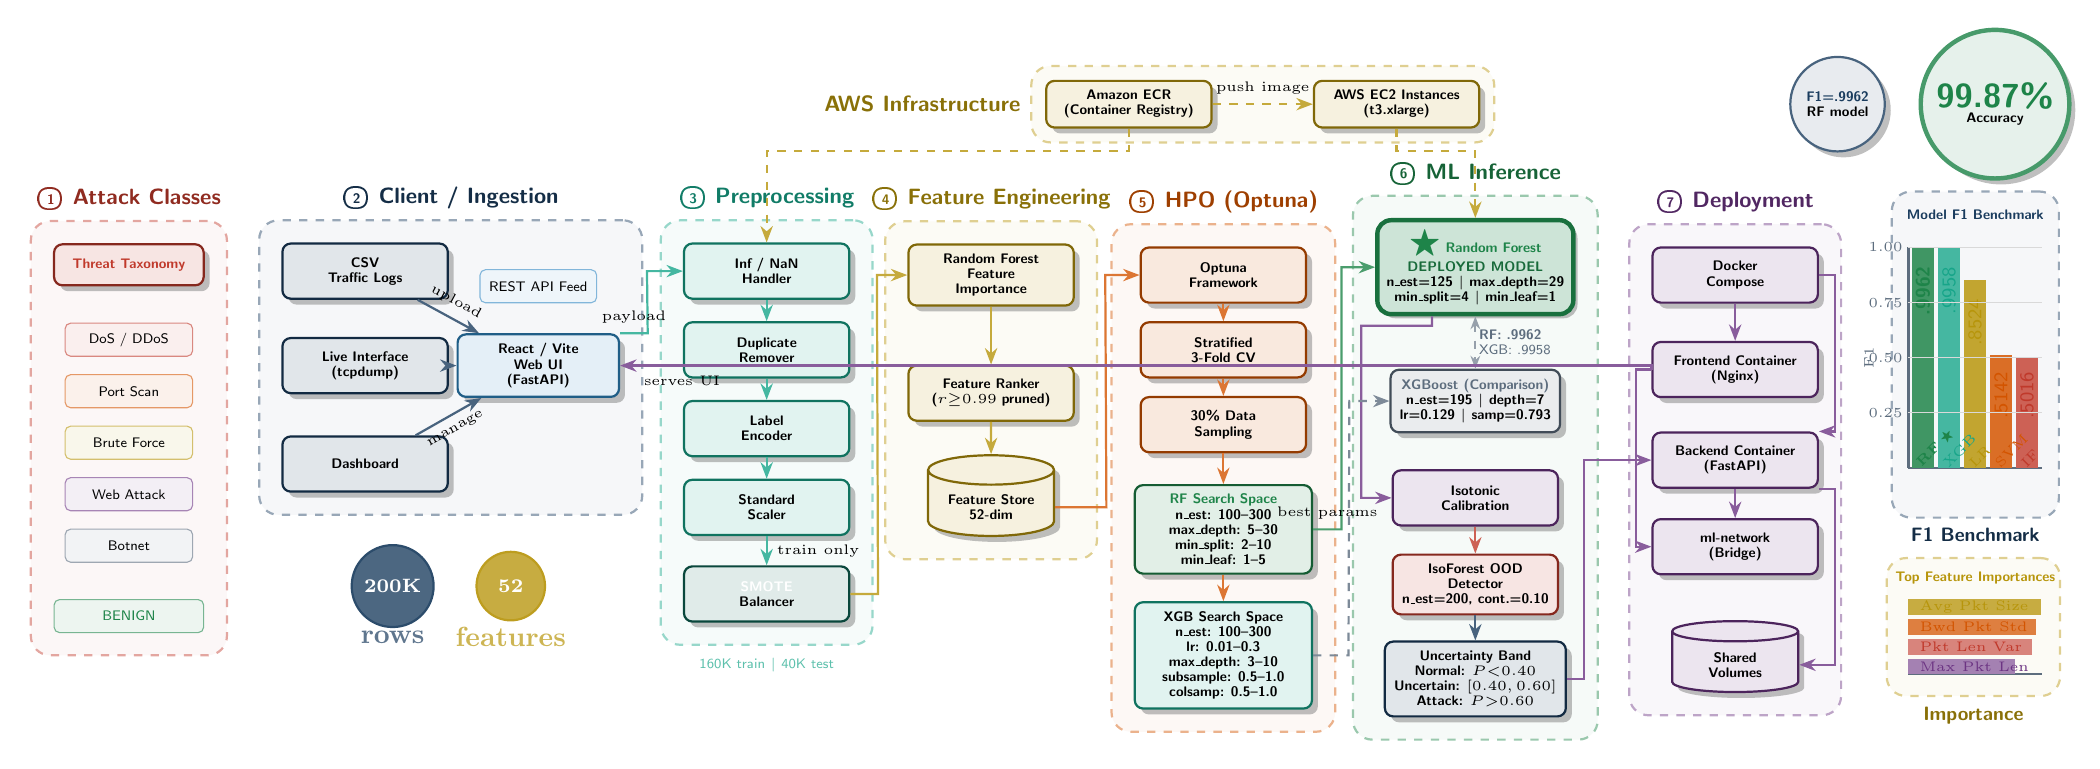
\begin{tikzpicture}[
  comp/.style={rectangle, draw=#1!70!black, thick, fill=#1!13,
               minimum width=2.1cm, minimum height=0.70cm,
               align=center, font=\sffamily\tiny\bfseries,
               rounded corners=3pt, drop shadow},
  compStar/.style={rectangle, draw=#1!85!black, ultra thick, fill=#1!22,
               minimum width=2.3cm, minimum height=0.86cm,
               align=center, font=\sffamily\tiny\bfseries,
               rounded corners=5pt,
               drop shadow={shadow xshift=1.5pt,shadow yshift=-1.5pt}},
  subnode/.style={rectangle, draw=#1!60, thin, fill=#1!8,
                  minimum width=1.4cm, minimum height=0.42cm,
                  align=center, font=\sffamily\tiny, rounded corners=2pt},
  db/.style={cylinder, draw=#1!70!black, thick, fill=#1!13,
             minimum width=1.6cm, minimum height=0.9cm,
             align=center, font=\sffamily\tiny\bfseries,
             shape border rotate=90, aspect=0.28, drop shadow},
  lane/.style={rectangle, draw=#1!45, dashed, thick,
               inner sep=8pt, fill=#1!4, rounded corners=7pt},
  laneLabel/.style={font=\sffamily\bfseries\scriptsize, text=#1!75!black},
  arr/.style={-{Stealth[scale=0.9]}, thick, draw=#1!80},
  arrD/.style={-{Stealth[scale=0.9]}, thick, draw=#1!80, dashed},
  arrC/.style={{Stealth[scale=0.7]}-{Stealth[scale=0.7]}, thick,
               draw=#1!65, dashed},
  stepBadge/.style={circle, fill=#1!78, draw=#1!92, thick,
                    minimum size=0.38cm, align=center,
                    font=\sffamily\bfseries\scriptsize, text=white}
]

% ===================================================
% ROW 0 — THREAT TAXONOMY
% ===================================================
\node[comp=clRed, minimum width=1.9cm, minimum height=0.52cm] (tax_title)
  at (-11.5, 3.58) {\color{clRed}Threat Taxonomy};

\node[subnode=clRed,    minimum width=1.62cm] (tax_dos)  [below=0.46cm of tax_title] {DoS / DDoS};
\node[subnode=clOrange, minimum width=1.62cm] (tax_port) [below=0.22cm of tax_dos]   {Port Scan};
\node[subnode=clGold,   minimum width=1.62cm] (tax_bf)   [below=0.22cm of tax_port]  {Brute Force};
\node[subnode=clPurple, minimum width=1.62cm] (tax_web)  [below=0.22cm of tax_bf]    {Web Attack};
\node[subnode=clGray,   minimum width=1.62cm] (tax_bot)  [below=0.22cm of tax_web]   {Botnet};
\node[subnode=clGreen,  minimum width=1.90cm] (tax_ben)  [below=0.46cm of tax_bot]
  {\color{clGreen}BENIGN};

\begin{scope}[on background layer]
  \node[lane=clRed,
        fit=(tax_title)(tax_dos)(tax_port)(tax_bf)(tax_web)(tax_bot)(tax_ben),
        label={[laneLabel=clRed]above:\footnotesize\textbf{\textcircled{\tiny 1}} Attack Classes}] {};
\end{scope}

% ===================================================
% ROW 1 — INGESTION / CLIENT LAYER
% ===================================================
\node[comp=clBlue] (csv)   at (-8.5, 3.50) {CSV\\Traffic Logs};
\node[comp=clBlue] (live)  at (-8.5, 2.30) {Live Interface\\(tcpdump)};
\node[comp=clBlue] (admin) at (-8.5, 1.05) {Dashboard};

\node[comp=clLightBlue, minimum width=2.05cm] (react)
                            at (-6.3, 2.30) {React / Vite\\Web UI\\(FastAPI)};
\node[subnode=clLightBlue] (ws)  [above=0.38cm of react] {REST API Feed};
% \node[subnode=clLightBlue] (vis) [below=0.38cm of react] {D3.js Visualiser};

\draw[arr=clBlue] (csv)   -- node[above,font=\tiny,sloped]{upload} (react);
\draw[arr=clBlue] (live)  -- (react);
\draw[arr=clBlue] (admin) -- node[below,font=\tiny,sloped]{manage} (react);

% Volume badge
\node[stepBadge=clBlue, minimum size=0.46cm] at (-8.15, -0.50) {\bf 200K};
\node[font=\sffamily, text=clBlue!70] at (-8.15, -1.15) {\bf rows};

\node[stepBadge=clGold, minimum size=0.87cm] at (-6.65, -0.50) {\bf 52};
\node[font=\sffamily, text=clGold!70] at (-6.65, -1.15) {\bf features};

\begin{scope}[on background layer]
  \node[lane=clBlue,
        fit=(csv)(live)(admin)(react)(ws),
        label={[laneLabel=clBlue]above:\footnotesize\textbf{\textcircled{\tiny 2}} Client / Ingestion}] (clientLane) {};
\end{scope}

% ===================================================
% ROW 2 — PREPROCESSING
% ===================================================
\node[comp=clCyan]  (inf)   at (-3.4, 3.50) {Inf / NaN\\Handler};
\node[comp=clCyan]  (dup)   at (-3.4, 2.50) {Duplicate\\Remover};
\node[comp=clCyan]  (enc)   at (-3.4, 1.50) {Label\\Encoder};
\node[comp=clCyan]  (scl)   at (-3.4, 0.50) {Standard\\Scaler};
\node[comp=clTeal]  (smote) at (-3.4,-0.60) {\color{white}SMOTE\\Balancer};

\draw[arr=clCyan]  (inf)   -- (dup);
\draw[arr=clCyan]  (dup)   -- (enc);
\draw[arr=clCyan]  (enc)   -- (scl);
\draw[arr=clCyan]  (scl)   -- node[right,font=\tiny]{train only} (smote);

\draw[arr=clCyan]
  (react.north east) -- node[above,font=\tiny]{payload} ++(0.35,0)
  -- (-4.92,3.50) -- (inf.west);

\node[font=\sffamily\tiny, text=clCyan!70] at (-3.4,-1.5)
  {160K train $\mid$ 40K test};

\begin{scope}[on background layer]
  \node[lane=clCyan,
        fit=(inf)(dup)(enc)(scl)(smote),
        label={[laneLabel=clCyan]above:\footnotesize\textbf{\textcircled{\tiny 3}} Preprocessing}] (prepLane) {};
\end{scope}

% ===================================================
% ROW 3 — FEATURE ENGINEERING
% ===================================================
\node[comp=clGold] (rffi) at (-0.55, 3.45)
  {Random Forest\\Feature\\Importance};
\node[comp=clGold] (ranker) at (-0.55, 1.95)
  {Feature Ranker\\($r{\ge}0.99$ pruned)};
\node[db=clGold]   (feat_store) at (-0.55, 0.50)
  {Feature Store\\{\tiny 52-dim}};

\draw[arr=clGold] (rffi)       -- (ranker);
\draw[arr=clGold] (ranker)     -- (feat_store);
\draw[arr=clGold]
  (smote.east) -- ++(0.35,0)
  -- (-2.0,3.45) -- (rffi.west);

\begin{scope}[on background layer]
  \node[lane=clGold,
        fit=(rffi)(ranker)(feat_store),
        label={[laneLabel=clGold]above:\footnotesize\textbf{\textcircled{\tiny 4}} Feature Engineering}] (featLane) {};
\end{scope}

% ===================================================
% ROW 4 — HPO
% ===================================================
\node[comp=clOrange] (hpo_title) at (2.4, 3.45) {Optuna\\Framework};
\node[comp=clOrange] (hpo_strat) at (2.4, 2.50) {Stratified\\3-Fold CV};
\node[comp=clOrange] (hpo_samp)  at (2.4, 1.55) {30\% Data\\Sampling};

\node[comp=clGreen, minimum width=2.25cm] (hpo_rf) at (2.4, 0.22)
  {\color{clGreen}RF Search Space\\{\tiny n\_est: 100--300}\\{\tiny max\_depth: 5--30}\\
   {\tiny min\_split: 2--10}\\{\tiny min\_leaf: 1--5}};

\node[comp=clCyan, minimum width=2.25cm] (hpo_xgb) at (2.4,-1.38)
  {XGB Search Space\\{\tiny n\_est: 100--300}\\{\tiny lr: 0.01--0.3}\\
   {\tiny max\_depth: 3--10}\\{\tiny subsample: 0.5--1.0}\\{\tiny colsamp: 0.5--1.0}};

\draw[arr=clOrange] (hpo_title) -- (hpo_strat);
\draw[arr=clOrange] (hpo_strat) -- (hpo_samp);
\draw[arr=clOrange] (hpo_samp)  -- (hpo_rf);
\draw[arr=clOrange] (hpo_rf)    -- (hpo_xgb);

\draw[arr=clOrange]
  (feat_store.east) -- ++(0.65,0)
  -- (0.9,3.45) -- (hpo_title.west);

\begin{scope}[on background layer]
  \node[lane=clOrange,
        fit=(hpo_title)(hpo_strat)(hpo_samp)(hpo_rf)(hpo_xgb),
        label={[laneLabel=clOrange]above:\footnotesize\textbf{\textcircled{\tiny 5}} HPO (Optuna)}] (hpoLane) {};
\end{scope}

% ===================================================
% ROW 5 — ML ENGINE
% ===================================================

% PRIMARY deployed model
\node[compStar=clGreen] (rf_main) at (5.6, 3.55)
  {\color{clGreen}{\large\bfseries\sffamily$\bigstar$} Random Forest\\
   {\tiny\color{clGreen!80!black}DEPLOYED MODEL}\\
   \tiny n\_est=125 $|$ max\_depth=29\\
   \tiny min\_split=4 $|$ min\_leaf=1};

% Comparison model (grayed)
\node[comp=clGray, minimum width=2.05cm] (xgb2) at (5.6, 1.85)
  {\color{clGray}XGBoost (Comparison)\\
   \tiny n\_est=195 $|$ depth=7\\
   \tiny lr=0.129 $|$ samp=0.793};

% Bi-directional comparison annotation
\draw[arrC=clGray] (rf_main.south) --
  node[right,font=\sffamily\tiny,text=clGray,align=left,inner sep=1pt]
    {\textbf{RF: .9962}\\XGB: .9958}
  (xgb2.north);

% Main flow: RF (skip xgb2) → calibrate → OOD → band
\node[comp=clPurple] (calib)  at (5.6, 0.62) {Isotonic\\Calibration};
\node[comp=clRed]    (ood)    at (5.6,-0.48)
  {IsoForest OOD\\Detector\\{\tiny n\_est=200, cont.=0.10}};
\node[comp=clBlue]   (thresh) at (5.6,-1.68)
  {Uncertainty Band\\{\tiny Normal: $P{<}0.40$}\\
   {\tiny Uncertain: $[0.40, 0.60]$}\\{\tiny Attack: $P{>}0.60$}};

% RF → calib bypass xgb2 (route left)
\draw[arr=clPurple]
  ([xshift=-0.55cm]rf_main.south) -- ++(0,-0.12) -- ++(-0.9,0)
  -- (-0.55+4.7, 0.62) -- (calib.west);
\draw[arr=clRed]    (calib)  -- (ood);
\draw[arr=clBlue]   (ood)    -- (thresh);

% HPO → RF  (from RF search space)
\draw[arr=clGreen]
  (hpo_rf.east) -- ++(0.36,0)
  node[midway,above,font=\tiny]{best params}
  -- (3.9,3.55) -- (rf_main.west);

% HPO → XGB comparison (dashed)
\draw[arrD=clGray]
  (hpo_xgb.east) -- ++(0.45,0) -- (4.0,1.85) -- (xgb2.west);

\begin{scope}[on background layer]
  \node[lane=clGreen,
        fit=(rf_main)(xgb2)(calib)(ood)(thresh),
        label={[laneLabel=clGreen]above:\footnotesize\textbf{\textcircled{\tiny 6}} ML Inference}] (mlLane) {};
\end{scope}

% ===================================================
% ROW 6 — DOCKERIZATION
% ===================================================
\node[comp=clPurple] (compose) at (8.9, 3.45) {Docker\\Compose};
\node[comp=clPurple] (c_front) at (8.9, 2.25) {Frontend Container\\(Nginx)};
\node[comp=clPurple] (c_back)  at (8.9, 1.10) {Backend Container\\(FastAPI)};
\node[comp=clPurple] (net)     at (8.9, 0.00) {ml-network\\(Bridge)};
\node[db=clPurple]   (vols)    at (8.9,-1.50) {Shared\\Volumes};

% PROD badge
% \node[stepBadge=clGreen, minimum size=0.52cm,
%       font=\sffamily\bfseries\tiny] at (10.05, 3.85) {\tiny\bf PROD};

\draw[arr=clPurple] (thresh.east) -- ++(0.22,0) |- (c_back.west);
\draw[arr=clPurple] (compose) -- (c_front);
\draw[arr=clPurple] (compose.east) -- ++(0.20,0) |- (c_back.north east);
\draw[arr=clPurple] (c_back)  -- (net);
\draw[arr=clPurple] (c_front.west) -- ++(-0.20,0) |- (net.west);
\draw[arr=clPurple] (c_back.south east) -- ++(0.20,0) |- (vols.east);

\draw[arr=clPurple]
  (c_front.west) |-
  node[pos=0.97,below,font=\tiny,align=center]{serves UI}
  (react.east);

\begin{scope}[on background layer]
  \node[lane=clPurple,
        fit=(compose)(c_front)(c_back)(net)(vols),
        label={[laneLabel=clPurple]above:\footnotesize\textbf{\textcircled{\tiny 7}} Deployment}] (dockerLane) {};
\end{scope}

% ===================================================
% AWS INFRA BAR
% ===================================================
\node[comp=clGold, minimum width=2.1cm, minimum height=0.46cm]
  (ecr) at (1.2, 5.62)
  {\tiny Amazon ECR\\(Container Registry)};
\node[comp=clGold, minimum width=2.1cm, minimum height=0.46cm]
  (ec2) at (4.6, 5.62)
  {\tiny AWS EC2 Instances\\(t3.xlarge)};

\draw[arrD=clGold] (ecr) -- node[above,font=\tiny]{push image} (ec2);

\begin{scope}[on background layer]
  \node[lane=clGold, inner sep=5pt,
        fit=(ecr)(ec2),
        label={[laneLabel=clGold]left:\footnotesize AWS Infrastructure}] (awsLane) {};
\end{scope}

\draw[arrD=clGold] (ecr.south) -- ++(0,-0.28) -| (inf.north);
\draw[arrD=clGold] (ec2.south) -- ++(0,-0.28) -| (rf_main.north);

% ===================================================
% RIGHT PANEL — F1 BENCHMARK BAR CHART
% ===================================================
\begin{scope}[shift={(11.1, 1.0)}]
  \node[font=\sffamily\tiny\bfseries, text=clBlue] at (0.85,3.22)
    {Model F1 Benchmark};

  \draw[thick, clGray] (0,0) -- (0,2.80);
  \draw[thick, clGray] (0,0) -- (1.70,0);
  \node[font=\tiny, rotate=90, text=clGray] at (-0.50,1.40) {F1};

  % Bars: F1 × 2.8
  \fill[clGreen!85]  (0.05,0) rectangle (0.32, 2.789);
  \fill[clCyan!80]   (0.38,0) rectangle (0.65, 2.788);
  \fill[clGold!85]   (0.71,0) rectangle (0.98, 2.387);
  \fill[clOrange!85] (1.04,0) rectangle (1.31, 1.440);
  \fill[clRed!80]    (1.37,0) rectangle (1.64, 1.405);

  \node[font=\sffamily\scriptsize\bfseries, text=clGreen,  rotate=90] at (0.185,2.25) {.9962};
  \node[font=\sffamily\scriptsize,          text=clCyan,   rotate=90] at (0.515,2.25) {.9958};
  \node[font=\sffamily\scriptsize,          text=clGold,   rotate=90] at (0.845,1.85) {.8524};
  \node[font=\sffamily\scriptsize,          text=clOrange, rotate=90] at (1.175,0.92) {.5142};
  \node[font=\sffamily\scriptsize,          text=clRed,    rotate=90] at (1.505,0.92) {.5016};

  \node[font=\tiny\bfseries, rotate=45, anchor=west, text=clGreen]  at (0.05,-0.05)  {RF\,{\tiny$\bigstar$}};
  \node[font=\tiny,           rotate=45, anchor=west, text=clCyan]   at (0.38,-0.05) {XGB};
  \node[font=\tiny,           rotate=45, anchor=west, text=clGold]   at (0.71,-0.05) {LR};
  \node[font=\tiny,           rotate=45, anchor=west, text=clOrange] at (1.04,-0.05) {SVM};
  \node[font=\tiny,           rotate=45, anchor=west, text=clRed]    at (1.37,-0.05) {IF};

  \foreach \y/\lbl in {0.70/0.25, 1.40/0.50, 2.10/0.75, 2.80/1.00}{
    \draw[gray!30, thin] (0,\y) -- (1.70,\y);
    \node[font=\tiny, text=clGray, anchor=east] at (0.05,\y) {\lbl};
  }

  \begin{scope}[on background layer]
    \node[lane=clBlue, inner sep=6pt,
          fit={(0,-0.42)(1.70,3.30)},
          label={[laneLabel=clBlue]below:\scriptsize F1 Benchmark}] {};
  \end{scope}
\end{scope}

% ===================================================
% RIGHT PANEL — FEATURE IMPORTANCE CHART
% ===================================================
\begin{scope}[shift={(11.1,-1.62)}]
  \node[font=\sffamily\tiny\bfseries, text=clGold] at (0.85,1.22)
    {Top Feature Importances};

  \draw[thick, clGray] (0,0) -- (1.70,0);

  % Bars normalised to max importance 0.0841, scaled to width 1.70
  \fill[clGold!78]   (0, 0.75) rectangle (1.682, 0.95); % Avg Pkt Size: 0.0841
  \fill[clOrange!75] (0, 0.50) rectangle (1.616, 0.70); % Bwd Pkt Std:  0.0809
  \fill[clRed!62]    (0, 0.25) rectangle (1.574, 0.45); % Pkt Len Var:  0.0787
  \fill[clPurple!62] (0, 0.00) rectangle (1.350, 0.20); % Max Pkt Len:  0.0676

  \node[font=\tiny, anchor=west, text=clGold]   at (0.02,0.85) {Avg Pkt Size};
  \node[font=\tiny, anchor=west, text=clOrange] at (0.02,0.60) {Bwd Pkt Std};
  \node[font=\tiny, anchor=west, text=clRed]    at (0.02,0.35) {Pkt Len Var};
  \node[font=\tiny, anchor=west, text=clPurple] at (0.02,0.10) {Max Pkt Len};

  \begin{scope}[on background layer]
    \node[lane=clGold, inner sep=5pt,
          fit={(-0.10,-0.10)(1.75,1.30)},
          label={[laneLabel=clGold]below:\scriptsize Importance}] {};
  \end{scope}
\end{scope}

% ===================================================
% RIGHT PANEL — CALIBRATED UNCERTAINTY BAND
% ===================================================
% \begin{scope}[shift={(11.1,-3.12)}]
%   \node[font=\sffamily\tiny\bfseries, text=clOrange] at (0.85,0.90)
%     {Calibrated Uncertainty Band};

%   % Zone fill: Normal [0,0.40) | Uncertain [0.40,0.60] | Attack (0.60,1.0]
%   % Mapped: 0.40→0.68, 0.60→1.02 on width 1.70
%   \fill[clGreen!48]  (0.00,0.38) rectangle (0.68,0.72);
%   \fill[clOrange!58] (0.68,0.38) rectangle (1.02,0.72);
%   \fill[clRed!48]    (1.02,0.38) rectangle (1.70,0.72);

%   \draw[clOrange!90, thick] (0.68,0.33) -- (0.68,0.77);
%   \draw[clOrange!90, thick] (1.02,0.33) -- (1.02,0.77);

%   \node[font=\sffamily\scriptsize, text=clGreen!80!black]  at (0.34,0.55) {Normal};
%   \node[font=\sffamily\scriptsize, text=clOrange!90!black] at (0.85,0.55) {Uncert.};
%   \node[font=\sffamily\scriptsize, text=clRed!80!black]    at (1.36,0.55) {Attack};

%   \node[font=\sffamily\scriptsize\bfseries, text=clOrange] at (0.68,0.20) {0.40};
%   \node[font=\sffamily\scriptsize\bfseries, text=clOrange] at (1.02,0.20) {0.60};
%   \node[font=\sffamily\scriptsize, text=clGray]            at (0.00,0.20) {0.0};
%   \node[font=\sffamily\scriptsize, text=clGray]            at (1.70,0.20) {1.0};

%   \draw[-{Stealth[scale=0.7]}, clGray, thin] (0.00,0.05) -- (1.72,0.05);
%   \node[font=\tiny, text=clGray, anchor=west] at (1.74,0.05) {$P(\text{att.})$};

%   \begin{scope}[on background layer]
%     \node[lane=clOrange, inner sep=5pt,
%           fit={(-0.10,0.00)(1.82,0.96)},
%           label={[laneLabel=clOrange]below:\scriptsize Prediction Gate}] {};
%   \end{scope}
% \end{scope}

% ===================================================
% PERFORMANCE BADGES
% ===================================================
\node[circle, draw=clGreen!82, ultra thick, fill=clGreen!11,
      minimum size=1.54cm, align=center, font=\sffamily\tiny\bfseries,
      drop shadow] at (12.20, 5.62)
  {\color{clGreen}\large\textbf{99.87\%}\\\tiny Accuracy};

\node[circle, draw=clBlue!80, thick, fill=clBlue!10,
      minimum size=1.20cm, align=center, font=\sffamily\tiny\bfseries,
      drop shadow] at (10.20, 5.62)
  {\color{clBlue}\textbf{F1=.9962}\\\tiny RF model};

\end{tikzpicture}
}
% \vspace{-7pt}
\caption{Full-stack end-to-end architecture.
  \textbf{\textcircled{\tiny 1}~Taxonomy:} Six CICIDS2017 attack classes.
  \textbf{\textcircled{\tiny 2}~Ingestion:} React/Vite dashboard with FastAPI REST gateway and D3.js visualisation.
  \textbf{\textcircled{\tiny 3}~Preprocessing:} Deterministic Inf/NaN elimination, deduplication, $z$-score scaling,
  and SMOTE class-balancing (train-only); stratified 160K/40K split.
  \textbf{\textcircled{\tiny 4}~Feature Engineering:} RF-importance ranking with Pearson pruning ($r\!\ge\!0.99$)
  retaining \textbf{52 features}; packet-size statistics dominate.
  \textbf{\textcircled{\tiny 5}~HPO (Optuna):} Stratified 3-fold CV on 30\% sample; RF space (n\_est, max\_depth,
  min\_split, min\_leaf); XGB space (n\_est, lr, max\_depth, subsample, colsample\_bytree); metric: macro F1.
  \textbf{\textcircled{\tiny 6}~ML Engine:} HPO-tuned Random Forest (\textbf{$\bigstar$~deployed}; n\_est\,=\,125,
  max\_depth\,=\,29, min\_split\,=\,4, min\_leaf\,=\,1) with XGBoost comparison; isotonic
  probability calibration; Isolation Forest OOD detector (n\_est\,=\,200, contamination\,=\,0.10);
  calibrated uncertainty band [0.40,\,0.60].
  \textbf{\textcircled{\tiny 7}~Deployment:} Docker Compose---Nginx (frontend) + FastAPI (backend)---over
  \texttt{ml-network} bridge and shared volumes; images pushed to Amazon ECR, served on
  AWS EC2 (t3.xlarge).
  \textbf{Right panels:} F1 benchmark across all models, top-4 feature importances,
  and calibrated confidence gate.}
\label{fig:architecture}
\end{figure*}

% ================================================================
%  BODY — 2-COLUMN
% ================================================================

% \vspace{-6pt}
\section{Introduction}
% \vspace{-3pt}
Modern adversarial traffic demands detection frameworks that are accurate, latency-sensitive, and operationally resilient. We address these constraints via a cloud-native deployment combining containerised microservices with an end-to-end automated ML pipeline, evaluated on the \textbf{CICIDS2017} benchmark---encompassing DoS, DDoS, port scans, brute-force, web-application, and botnet vectors.

% \vspace{-5pt}
\section{Methodology}
% \vspace{-3pt}

\subsection{Cloud-Native Architecture}
The system adopts a three-tier model: (i)~a React/Vite dashboard with an integrated FastAPI backend, providing interactive visualisation via a REST API; (ii)~a FastAPI gateway with Pydantic schema enforcement, CORS middleware, and a 50\,MB file gate, returning three-class verdicts (\textit{Normal}, \textit{Uncertain}, \textit{Attack}); and (iii)~an ML runtime on AWS EC2 (\texttt{t3.xlarge}) provisioned through Amazon ECR. The stack is containerised via Docker Compose---Nginx frontend and FastAPI backend over \texttt{ml-network} bridge with shared volumes.

\subsection{ML Pipeline}
\textbf{Preprocessing:} CICFlowMeter features are deterministically cleaned (inf/NaN clipped, duplicates removed). A stratified 80/20 split is applied to a 200K-row working set; features are $z$-score normalised; SMOTE balances the training partition only.\\ \\
\hspace*{\parindent}\textbf{Feature selection:} Pearson pruning ($r\!\ge\!0.99$) eliminates redundant dimensions; an RF importance sweep ranks all 52 retained features, dominated by packet-size statistics.\\ \\
\hspace*{\parindent}\textbf{HPO:} Optuna maximises macro F1 under stratified 3-fold CV on 30\% of training data. RF search: n\_est\,$\in[100,300]$, max\_depth\,$\in[5,30]$, min\_split\,$\in[2,10]$, min\_leaf\,$\in[1,5]$. XGBoost adds lr\,$\in[0.01,0.3]$, subsample\,$\in[0.5,1.0]$, colsample\_bytree\,$\in[0.5,1.0]$.\\ \\
\hspace*{\parindent}\textbf{Calibration \& OOD:} Class probabilities are isotonically recalibrated. An Isolation Forest OOD detector (n\_est\,=\,200, contamination\,=\,0.10) on normal-only data flags distribution-shifted inputs; the uncertainty band $[0.40,\,0.60]$ abstains rather than forcing a binary verdict. \\

% \vspace{-5pt}
\section{Results}
% \vspace{-2pt}

\begin{table}[!h]
% \vspace{-6pt}
\caption{Model Performance Comparison (CICIDS2017 Held-Out Test Set)}
% \vspace{-4pt}
\begin{center}
\setlength{\tabcolsep}{4.0pt}
\begin{tabular}{l r r r r}
\toprule
\textbf{Model} & \textbf{Acc.} & \textbf{Prec.} & \textbf{Rec.} & \textbf{F1} \\
\midrule
\textbf{Random Forest (ours)} & \textbf{.9987} & .9957 & .9966 & \textbf{.9962} \\
XGBoost                       & .9986          & .9926 & .9990 & .9958 \\
Logistic Regression           & .9437          & .7649 & .9625 & .8524 \\
One-Class SVM                 & .7986          & .4338 & .6312 & .5142 \\
Isolation Forest              & .7961          & .4270 & .6078 & .5016 \\
\bottomrule
\end{tabular}
\label{tab:models}
\end{center}
% \vspace{-8pt}
\end{table}

Random Forest outperforms all baselines. Its precision edge over XGBoost (+0.31\,pp) reflects superior false-alarm resistance under class imbalance. Logistic Regression's precision shortfall ($\Delta\!=\!0.23$) exposes the inadequacy of linear boundaries on high-dimensional traffic manifolds. Unsupervised baselines (One-Class SVM, Isolation Forest) near chance, confirming the necessity of fully supervised training.

% \vspace{-5pt}
\section{Conclusion}
% \vspace{-3pt}
We deliver a production-ready NIDS achieving \textbf{99.87\% accuracy} and \textbf{F1\,=\,0.9962} on CICIDS2017. Its modular architecture---SMOTE-balanced preprocessing, RF-ranked 52-feature selection, Optuna HPO, isotonic calibration, and Isolation Forest OOD gating with a calibrated uncertainty band [0.40,\,0.60]---establishes a robust template for real-time cloud-scale cyber-threat mitigation.

\vspace{5pt}
\noindent\textbf{System URL: \href{http://54.198.216.48:3000/}{http://54.198.216.48:3000/}}

\end{document}
